\begin{figure}[htbp]\centering
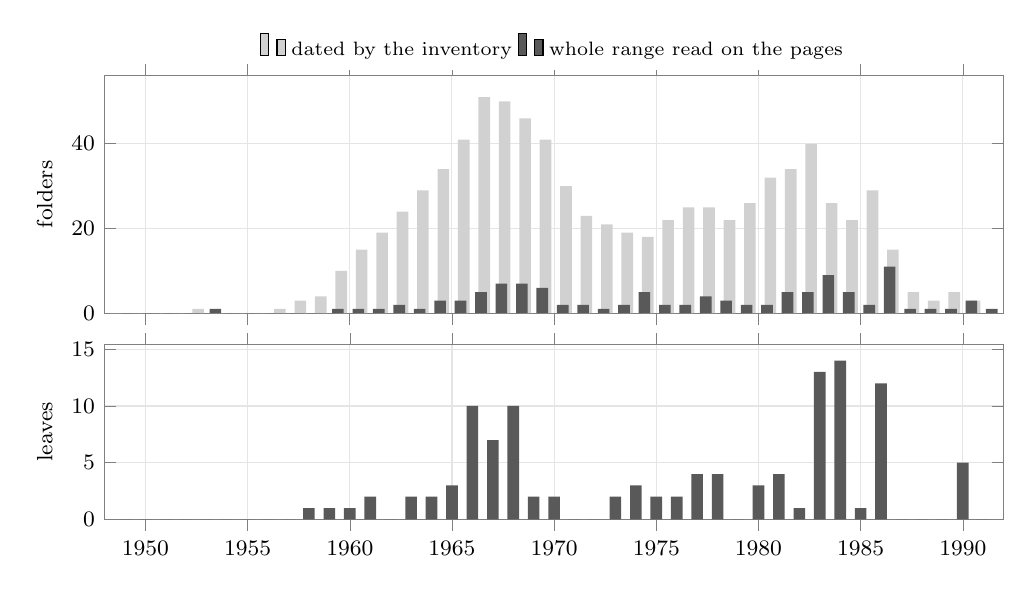
\begin{tikzpicture}
\begin{axis}[name=top,width=13cm,height=4.6cm,xmin=1948,xmax=1992,ymin=0,
  xticklabels={},ylabel={folders},ybar,bar width=4.2pt,grid=major,grid style={black!10},
  tick label style={font=\footnotesize},label style={font=\footnotesize},axis line style={black!50},
  legend style={font=\scriptsize,draw=none,at={(0.5,1.02)},anchor=south},legend columns=2,legend cell align=left]
\addplot[fill=black!18,draw=none] coordinates {(1949,0) (1950,0) (1951,0) (1952,0) (1953,1) (1954,0) (1955,0) (1956,0) (1957,1) (1958,3) (1959,4) (1960,10) (1961,15) (1962,19) (1963,24) (1964,29) (1965,34) (1966,41) (1967,51) (1968,50) (1969,46) (1970,41) (1971,30) (1972,23) (1973,21) (1974,19) (1975,18) (1976,22) (1977,25) (1978,25) (1979,22) (1980,26) (1981,32) (1982,34) (1983,40) (1984,26) (1985,22) (1986,29) (1987,15) (1988,5) (1989,3) (1990,5) (1991,3)};
\addplot[fill=black!65,draw=none] coordinates {(1949,0) (1950,0) (1951,0) (1952,0) (1953,1) (1954,0) (1955,0) (1956,0) (1957,0) (1958,0) (1959,1) (1960,1) (1961,1) (1962,2) (1963,1) (1964,3) (1965,3) (1966,5) (1967,7) (1968,7) (1969,6) (1970,2) (1971,2) (1972,1) (1973,2) (1974,5) (1975,2) (1976,2) (1977,4) (1978,3) (1979,2) (1980,2) (1981,5) (1982,5) (1983,9) (1984,5) (1985,2) (1986,11) (1987,1) (1988,1) (1989,1) (1990,3) (1991,1)};
\legend{dated by the inventory, whole range read on the pages}
\end{axis}
\begin{axis}[at={(top.south)},anchor=north,yshift=-4mm,width=13cm,height=3.8cm,xmin=1948,xmax=1992,ymin=0,
  ylabel={leaves},ybar,bar width=4.2pt,grid=major,grid style={black!10},xtick={1950,1955,1960,1965,1970,1975,1980,1985,1990},
  x tick label style={/pgf/number format/1000 sep={}},
  tick label style={font=\footnotesize},label style={font=\footnotesize},axis line style={black!50}]
\addplot[fill=black!65,draw=none] coordinates {(1949,0) (1950,0) (1951,0) (1952,0) (1953,0) (1954,0) (1955,0) (1956,0) (1957,0) (1958,1) (1959,1) (1960,1) (1961,2) (1962,0) (1963,2) (1964,2) (1965,3) (1966,10) (1967,7) (1968,10) (1969,2) (1970,2) (1971,0) (1972,0) (1973,2) (1974,3) (1975,2) (1976,2) (1977,4) (1978,4) (1979,0) (1980,3) (1981,4) (1982,1) (1983,13) (1984,14) (1985,1) (1986,12) (1987,0) (1988,0) (1989,0) (1990,5) (1991,0)};
\end{axis}
\end{tikzpicture}
\caption{Two kinds of date on one axis, each on its own scale. Above: for each year, how many of the 153 dated folders the inventory's ranges cover (an open end, « à partir de 1982 », counted five years on), and, darker, how many of them rest on a range the archivists read on the pages rather than deduced in their square brackets; 25 folders are « s.d. ». Below: the 113 dates the transcriptions have found written on the leaves themselves, machine stamps on reused paper left out. From \texttt{src/content/catalogue.ts} and \texttt{src/content/dated-leaves.json} (2026-09-26), after the site's page \emph{Timeline}.}\label{fig:dating}
\end{figure}
